\providecommand{\main}{..}
\documentclass[\main/main.tex]{subfiles}
\colorlet{punct}{red!60!black}
\definecolor{background}{HTML}{EEEEEE}
\definecolor{delim}{RGB}{20,105,176}
\colorlet{numb}{magenta!60!black}
\lstdefinelanguage{json}{
    basicstyle=\normalfont\ttfamily,
    numbers=left,
    numberstyle=\scriptsize,
    stepnumber=1,
    numbersep=8pt,
    showstringspaces=false,
    breaklines=true,
    frame=lines,
    backgroundcolor=\color{background},
    literate=
     *{0}{{{\color{numb}0}}}{1}
      {1}{{{\color{numb}1}}}{1}
      {2}{{{\color{numb}2}}}{1}
      {3}{{{\color{numb}3}}}{1}
      {4}{{{\color{numb}4}}}{1}
      {5}{{{\color{numb}5}}}{1}
      {6}{{{\color{numb}6}}}{1}
      {7}{{{\color{numb}7}}}{1}
      {8}{{{\color{numb}8}}}{1}
      {9}{{{\color{numb}9}}}{1}
      {:}{{{\color{punct}{:}}}}{1}
      {,}{{{\color{punct}{,}}}}{1}
      {\{}{{{\color{delim}{\{}}}}{1}
      {\}}{{{\color{delim}{\}}}}}{1}
      {[}{{{\color{delim}{[}}}}{1}
      {]}{{{\color{delim}{]}}}}{1},
}

\begin{document}
\chapter{Architecture}

\section{Software architecture}
The \emph{software architecture} of a system depicts the system’s organization or structure, and provides an explanation of how it behaves. A system represents the collection of components that accomplish a specific function or set of functions. In other words, the software architecture provides a sturdy foundation on which software can be built. A series of architecture decisions and trade-offs impact quality, performance, maintainability, and overall success of the system. \cite{Perry1992FoundationsFT} \cite{sw_arch_synopsys}. There are three different classes of architectural elements: 
\begin{enumerate}
    \item \textbf{Processing elements}: elements that supply the transformation on data elements;
    \item \textbf{Data elements}: elements that contain the information that is used and transformed;
    \item \textbf{Connecting elements}: elements that connect different architectural elements together.
\end{enumerate}
The architectural form consists of weighted properties and relationships, where the weight indicates either the importance of the property/relationship, or the necessity to select among alternatives, some of which may be preferred over others. The so called \emph{Architect} is able to distinguish between important and decorative formal aspects using properties and relationships weights. These aspects, carefully chosen and designed by the architect, are the key to achieving and reasoning about the system’s design goals \cite{sw_arch_def_carnegie}. 
\section{Service-Oriented Architecture}
Service-Oriented Architecture (SOA) is an architectural style that supports service-orientation. Service-orientation is a way of thinking in terms of services and service-based development and the outcomes of services \cite{soa_definition}. The SOA architectural style has the following distinctive features:
\begin{enumerate}
    \item it is based on the design of the services – which mirror real-world business activities – comprising the enterprise (or inter-enterprise) business processes;
    \item service representation implements services using service orchestration;
    \item it places unique requirements on the infrastructure;
    \item implementations are environment-specific;
    \item it requires strong governance of service representation and implementation.
\end{enumerate}
A service:
\begin{enumerate}
    \item is a logical representation of a repeatable business activity that has a specified outcome (e.g., check customer credit, provide weather data, consolidate drilling reports);
    \item is self-contained;
    \item may be composed of other services;
    \item is a “black box” to consumers of the service.
\end{enumerate}

\section{Project architecture}
The implemented architecture follows the idea of SOA. It's based on a series of services that read the input and write the result on the data lake. The final result is a pipeline of services, executed one after the other.
\begin{figure}[H]
    \centering
    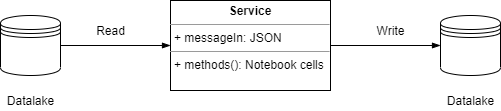
\includegraphics[width=\textwidth]{images/architecture/architecture_service_example.png}
    \caption{Architecture example}
    \label{fig:architecture_example}
\end{figure}
Every service executed is a transaction, if there is an error in the execution there's no update in written data. Reading and writing to disk is the most efficient approach, because it avoids to break the memory managing big datasets. 

\subsection{Categories of services}
In the implemented framework there are two main categories of services.
\begin{enumerate}
    \item \textbf{Preprocessing services}: preprocessing services are services that prepare the dataset to be used. Those services cover the corrective operations that are applied on the original dataset: textual data are cleaned from special characters, documents are adapted in order to be used further on, documents are filtered given a condition, and so on.  \\
    In this category there are two services: \emph{cleaning} and \emph{filtering} services.
    \item \textbf{Processing services}: processing services are services that constitutes the core of the framework: in those services, data is processed in order to produce usable embedding representation in order to perform a scoring algorithm to fulfill a semantic similarity search task. \\
    In this category there are three services: \emph{embedding extraction}, \emph{numerosity reduction} and \emph{scoring} services.
\end{enumerate}
\newpage
\subsection{DAG}
Once defined the services that need to be executed, these make up a so called Direct Acyclical Graph of execution: it consists of a pipeline where the result of a service execution is the input for the subsequent service. Ideally, the correct form of the DAG is visible in Figure \ref{fig:dag_example}:
\begin{figure}[H]
    \centering
    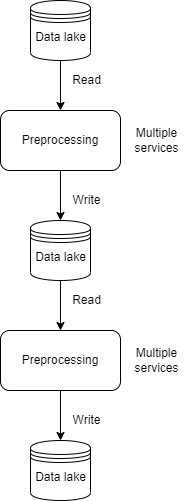
\includegraphics[scale=.68]{images/architecture/dag_theory.png}
    \caption{DAG example}
    \label{fig:dag_example}
\end{figure}
The two phases (\emph{preprocessing} and \emph{processing}), as visible in Figure \ref{fig:dag_example}, are subsequent and linked. If anything breaks the pipeline, the dataset will be updated to the last written result, allowing to restart from that checkpoint and not recomputing from the beginning, saving up precious machine-time.
\subsection{Orchestrator}
An orchestrator is a module of a framework which has the task of managing the execution of other modules in order to guarantee the right pipeline steps execution order. The orchestrator reads a series of messages that parametrize different services, than executes the associated services passing read messages as service input. Every message is a correctly formatted JSON object which contains all values that are necessary. An example of a message used as parameter for a service is visible in Listing \ref{parameter_message}.

\begin{center}
    \begin{lstlisting}[language=json, caption="Parameter message example", captionpos=b, label={parameter_message}]
        {
         "service_name": "test_service",
         "parameter_0": "value",
         "parameter_1": "value",
         ...,
         ...,
         "parameter_n": "value,
         "hyperparameters": ["hyperparameter_0", 
                             "hyperparameter_1", 
                             ..., 
                             "hyperparameter_m"]
        }
    \end{lstlisting}
\end{center}

Each of the above parameters and hyperparameters are passed to the associated service in order to instantiate different variables that will drive the service execution.
The pseudocode for the orchestrator is shown in Algorithm \ref{alg_orchestrator}.
\begin{center}
    \begin{algorithm}[H]
     \KwData{List of JSON messages}
     \KwResult{Execution of services}
     initialization\;
     \While{not at end of message list}{
      read message\;
      call right service\;
      pass current message as input\;
     }
    \caption{Orchestrator pseudocode}
    \label{alg_orchestrator}
    \end{algorithm}
    
\end{center}

\end{document}